%
% $Id: $
%
%
% Compilar a .pdf con LaTeX (pdflatex)
% Es necesario instalar Beamer (paquete latex-beamer en Debian)
%

%
% Gr�ficos:
% Los gr�ficos pueden suministrarse en PNG, JPG, TIF, PDF, MPS
% Los EPS deben convertirse a PDF (usar epstopdf)
%

\documentclass{beamer}
\usetheme{Warsaw}
%\usebackgroundtemplate{
\includegraphics[width=\paperwidth]{format/libresoft-bg.png}}
%\usepackage[spanish]{babel}
\usepackage[latin1]{inputenc}
\usepackage{graphics}
\usepackage{amssymb} % Simbolos matematicos
\usepackage{url}

%\definecolor{libresoftgreen}{RGB}{162,190,43}
%\definecolor{libresoftblue}{RGB}{0,98,143}

%\setbeamercolor{titlelike}{bg=libresoftgreen}

%% Metadatos del PDF.
\hypersetup{
  pdftitle={Can we Measure Computational Thinking with Tools? Present and Future of Dr. Scratch},
  pdfauthor={Jes�s Moreno Le�n, Gregorio Robles, Marcos Rom\'an-Gonz\'alez},
  pdfcreator={GSyC/LibreSoft \\ Universidad Rey Juan Carlos},
  pdfproducer=PDFLaTeX,
  pdfsubject={Computational Thinking. Automatic assessment with Dr. Scratch.},
}
%%

\begin{document}

\title{Can we Measure Computational Thinking with Tools? Present and Future of Dr. Scratch}
\institute{jesus.moreno@programamos.es, grex@gsyc.urjc.es, mroman@edu.uned.es \\
GSyC/Libresoft, Universidad Rey Juan Carlos}
\author{Jes�s Moreno-Le�n, Gregorio Robles \& Marcos Rom\'an-Gonz\'alez}
\date{SATToSE: Seminar Series on Advanced Techniques \& Tools for Software Evolution \\ Madrid. June 7, 2017}

\frame{
\maketitle
\begin{center}

\includegraphics[width=2cm]{format/libresoft-logo}
\hspace{0.5cm}

\includegraphics[width=5cm]{format/gsyc-urjc}
\vspace{0.5cm}

\includegraphics[width=3cm]{format/emadrid.png}
\end{center}
}


% Si el titulo o el autor se quieren acortar para los pies de p�gina
% se pueden redefinir aqu�:
\title{Present and Future of Dr. Scratch}
\author{J. Moreno-Le�n, G. Robles \& M. Rom\'an-Gonz\'alez}

%% LICENCIA DE REDISTRIBUCION DE LAS TRANSPAS
\frame{
~
\vspace{3cm}

\begin{flushright}

\includegraphics[width=2.2cm]{figs/by-sa}

{\tiny
(cc) 2017 Jes�s Moreno Le�n, Gregorio Robles and Marcos Rom\'an Gonz\'alez\\
  Some rights reserved. This work licensed under Creative Commons \\
  Attribution-ShareAlike License. To view a copy of full license, see \\
  http://creativecommons.org/licenses/by-sa/3.0/ or write to \\
  Creative Commons, 559 Nathan Abbott Way, Stanford, \\
  California 94305, USA. \\
\ \\
Some of the figures have been taken from the Internet \\
Source, and author and licence if known, is specified. \\
For those images, \emph{fair use} applies.
}
\end{flushright}
}
%%

\section{SATToSE 17, Madrid}


%--------------------------------------------------------
%\usebackgroundtemplate{
\includegraphics[width=10cm]{figs/drscratch1}}

\begin{frame}
\frametitle{What is Dr. Scratch?}

\begin{figure}[t!]
\begin{center}

\includegraphics[width=9cm]{figs/drscratch1.png}
\end{center}
\label{fig:naming}
\end{figure}

\end{frame}

%--------------------------------------------------------
%\usebackgroundtemplate{
\includegraphics[width=10cm]{figs/drscratch1}}

\begin{frame}
\frametitle{Why automatic analysis? (Learner perspective)}

\begin{figure}[t!]
\begin{center}
\begin{center}

\includegraphics[width=11cm]{figs/pylint.png}
\end{center}
Analyzing a Python program with Pylint
\end{center}
\end{figure}

\end{frame}

%--------------------------------------------------------
%\usebackgroundtemplate{
\includegraphics[width=10cm]{figs/drscratch1}}

\begin{frame}
\frametitle{Why automatic analysis? (Teacher perspective)}

\begin{figure}[t!]
\begin{center}
\begin{center}

\includegraphics[width=6cm]{figs/face.jpg}
\end{center}
Enjoying while marking students' projects
\end{center}
\label{fig:naming}
\end{figure}

\end{frame}

%--------------------------------------------------------
%\usebackgroundtemplate{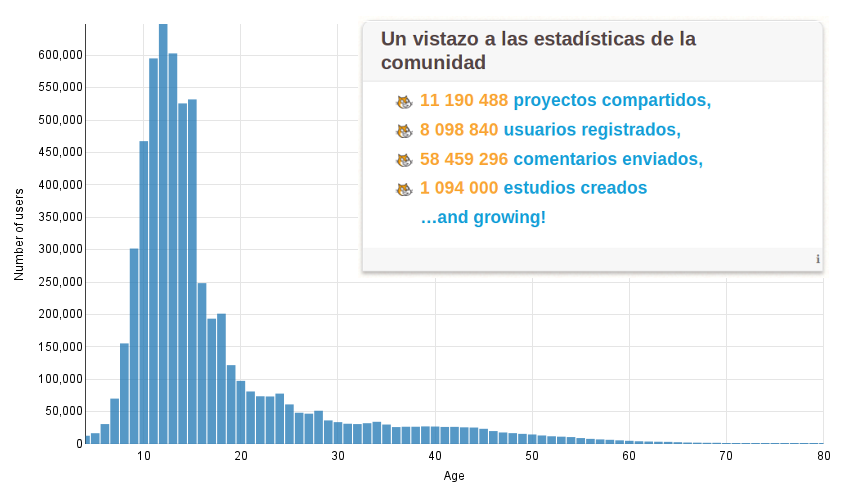
\includegraphics[width=18cm]{figs/stats.png}}

\begin{frame}
\frametitle{Remixing other researchers' ideas}
\begin{columns}[T]
    \begin{column}{1\textwidth}
     \begin{block}{Analysis of Scratch projects}
       \begin{itemize}
	 \item \texttt{Scrape}: visual representation of the blocks used (and not used).
         \item \texttt{Hairball}: static analyzer of Scratch projects to detect errors.
         \item Brennan \& Resnick: New frameworks for studying and assessing the development of CT.
         \item Seiter \& Foreman: Progression of Early CT Model.
         \item Wilson, Hainey \& Connolly: Evaluation of games to gauge understanding of programming concepts.
         %\item Koh, Basawapatna, Bennett, \& Repenning: Towards the Automatic Recognition of Computational Thinking for Adaptive Visual Language Learning
       \end{itemize}
    \end{block}
    \end{column}
  \end{columns}
\end{frame}

\usebackgroundtemplate{}

%--------------------------------------------------------
%\usebackgroundtemplate{\includegraphics[width=13cm]{figs/iceberg.jpg}}
% background: http://www.wim-network.org/wp-content/uploads/2012/04/iceberg.jpg

\begin{frame}
\frametitle{Assessment of CT development}
\begin{table}[t]\tiny 
\centering
%\begin{tabular}{p{2.5cm}p{2.7cm}p{3cm}p{4cm}}
\begin{tabular}{|p{2cm}|p{2cm}|p{2cm}|p{2cm}|}
%\toprule
\hline
{\bf CT dimension} & {\bf Basic} & {\bf Intermediate} & {\bf Proficient}\\ %\midrule 
\hline
Logical Thinking & if & if else & logic operations \\ \hline  
Data representation & modifiers of object properties & variables & lists  \\ \hline 
User interactivity & green flag & keyboard, mouse, ask and wait & webcam, input sound \\  \hline 
Control flow & sequence of blocks & repeat, forever & repeat until \\ \hline 
Abstraction and problem decomposition& more than one script & use of custom blocks & use of 'clones' (instances of sprites)\\ \hline 
Parallelism & two scripts on green flag & two scripts on key pressed or sprite clicked & two scripts on receive message, video/audio input, backdrop change \\ \hline 
Synchronization & wait & message broadcast, stop all, stop program & wait until, when backdrop changes to, broadcast and wait \\ 
\hline
\end{tabular}
\caption{Level of development for each CT dimension}
\label{table:CTscore}
\end{table}

\end{frame}

%--------------------------------------------------------
\begin{frame}
\frametitle{Assessment of CT development: Logical Thinking}

\begin{figure}[t!]
\begin{center}
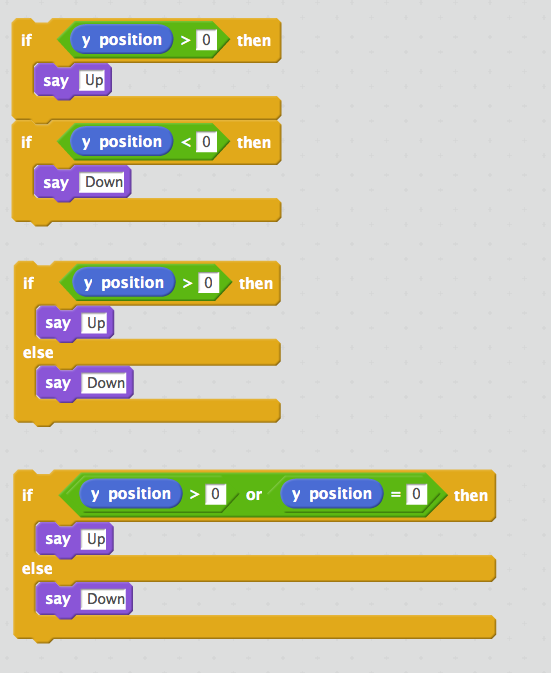
\includegraphics[height=6cm]{figs/Logic.png}
\end{center}
\label{fig:logic}
\end{figure}

\begin{center}
Different levels of development of logical thinking: basic (top), developing (center) and proficient (bottom).
\end{center}
\end{frame}

%--------------------------------------------------------
\begin{frame}
\frametitle{Assessment of CT development: Data Representation}

\begin{figure}[t!]
\begin{center}
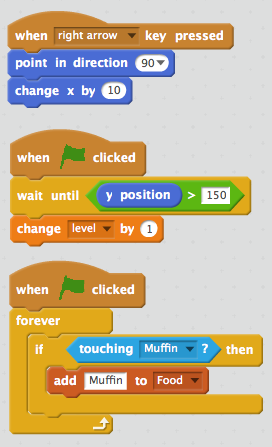
\includegraphics[height=6cm]{figs/Data.png}
\end{center}
\label{fig:logic}
\end{figure}

\begin{center}
Different levels of development of data representation: basic (top), developing (center) and proficient (bottom).
\end{center}
\end{frame}

%--------------------------------------------------------
\usebackgroundtemplate{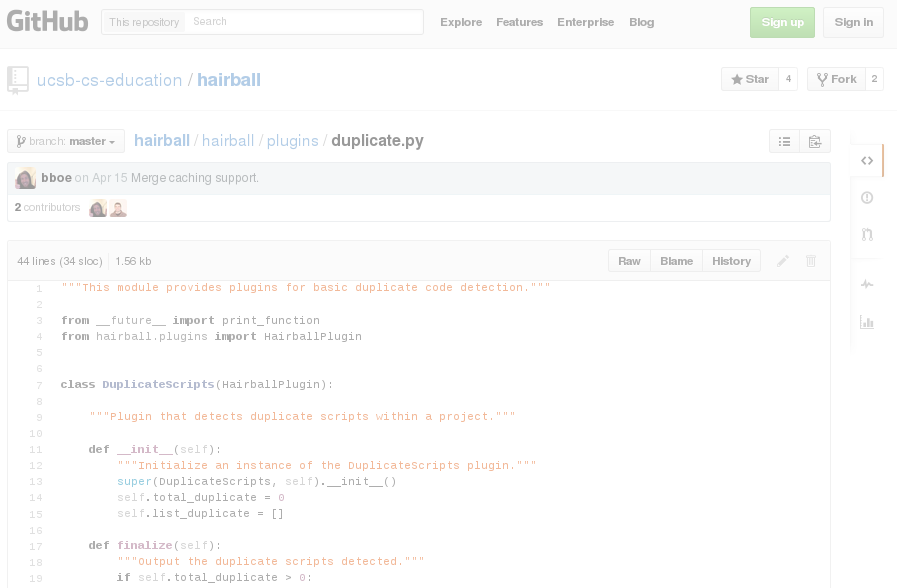
\includegraphics[width=13cm,height=9.2cm]{figs/plugins.png}}
\begin{frame}
\frametitle{Code smells (I)}
\begin{columns}[T]
    \begin{column}{0.8\textwidth}
     \begin{block}{Errors or bad programming habits}
\begin{itemize}
  \item Dead code
  \item Attribute initialization
  \item Default names
  \item Repeated scripts
\end{itemize}
    \end{block}
    \end{column}
  \end{columns}
\end{frame}

\usebackgroundtemplate{}
%--------------------------------------------------------
\begin{frame}
\frametitle{Code smells (II)}

\begin{figure}[t!]
\begin{center}
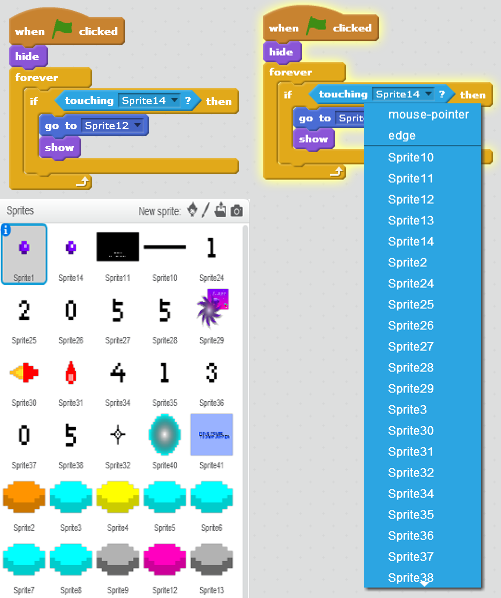
\includegraphics[width=7cm, height=6cm]{figs/SpriteNaming.png}
\end{center}
\label{fig:naming}
\end{figure}

\begin{center}
\emph{Bad}/default naming of sprites
\end{center}
\end{frame}

\usebackgroundtemplate{}
%--------------------------------------------------------

\begin{frame}
\frametitle{Code smells (and III)}

  \begin{columns}[T]
    \begin{column}{0.5\textwidth}
 
     \begin{block}{Example of repeated code}
\begin{figure}[t!]
\begin{center}
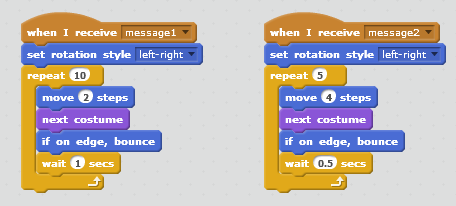
\includegraphics[width=5.4cm,height=2.5cm]{figs/CodeRepetition1.png}
\end{center}
\label{fig:repetition1}
\end{figure}
     \end{block}
    \end{column}
    \begin{column}{0.5\textwidth}
     \begin{block}{Solution to avoid repeated code}
\begin{figure}[t!]
\begin{center}
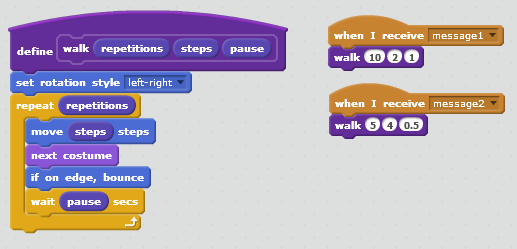
\includegraphics[width=5.4cm,height=2.5cm]{figs/CodeRepetition2.png}
\end{center}
Blocks should be created to avoid repetition of code
\label{fig:repetition2}
\end{figure}
     \end{block}

    \end{column}
  \end{columns}

\end{frame}

\usebackgroundtemplate{}

%--------------------------------------------------------

% \begin{frame}
% \frametitle{Scratch projects repository analysis}
% 
% \begin{table}
% \begin{center}
%   \begin{tabular}{ | l | c | c | c |}
%    \hline
%               & Default names & Duplicated scripts & Defined blocks \\ \hline\hline
%     Projects & 79 & 62 & 17 \\ \hline
%     Mean & 5.94 & 7.23 & 1.11 \\ \hline
%     Median & 3 & 2 & 0 \\ \hline
%     Maximum & 67 & 71 & 25 \\
%     \hline    
%   \end{tabular}
% \end{center}
% \caption{Analysis of 100 ramdonly downloaded Scratch projects}
% \label{table:results}
% \end{table}
% \end{frame}

%\usebackgroundtemplate{}
%--------------------------------------------------------
\usebackgroundtemplate{
\includegraphics[width=14cm]{figs/goals.jpg}}
%https://rebel-performance.com/wp-content/uploads/2014/10/goals.jpg

\begin{frame}
\frametitle{Goals}

\begin{itemize}
\item \Large  {\bf Review the current state of the validation process of the tool}\\
\item \Large  {\bf Show examples to illustrate the kind of software evolution investigations that could be performed using the tool}
\end{itemize}
\hfill{\Tiny Background picture: rebel-performance.com}
\end{frame}

\usebackgroundtemplate{}
%----------------------------------------------------

\usebackgroundtemplate{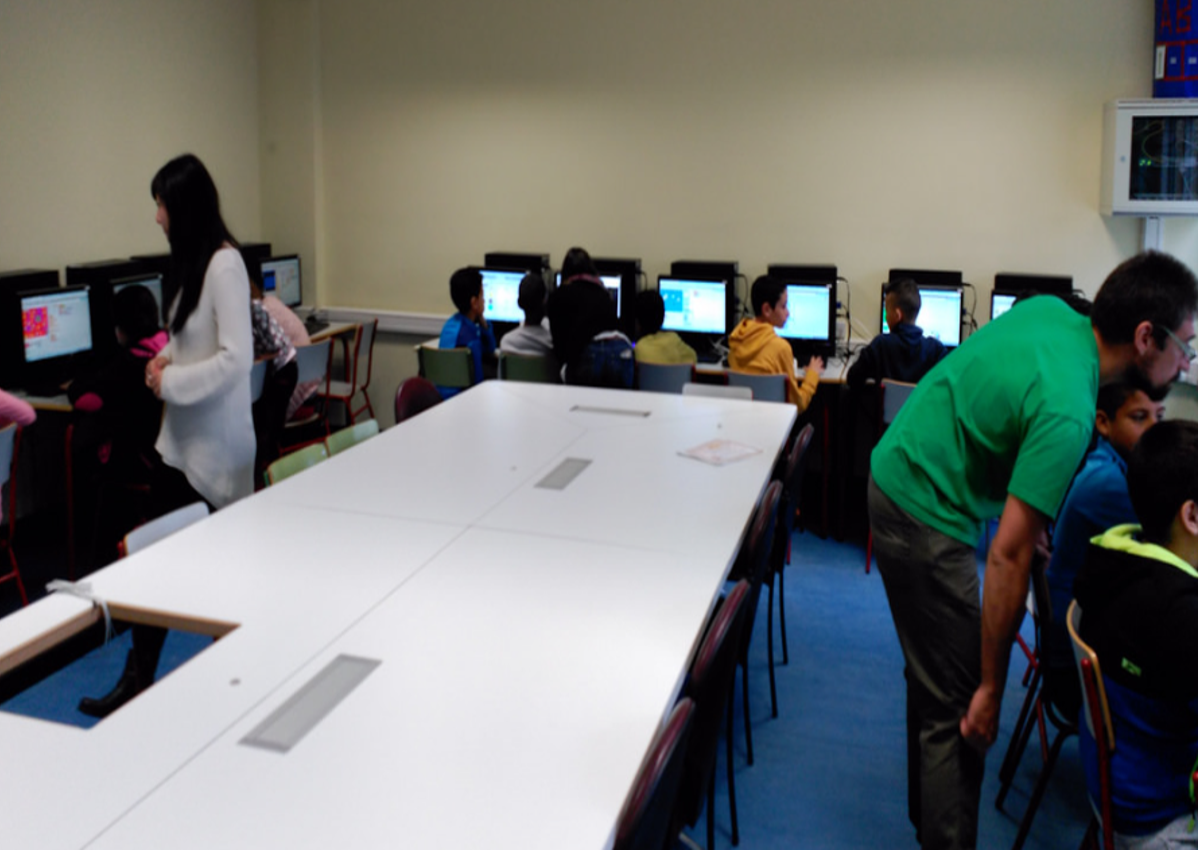
\includegraphics[width=13cm]{figs/colegio.png}}
\begin{frame}
\frametitle{Validation Process: Ecological Validity (I)}
\begin{columns}[T]
    \begin{column}{0.8\textwidth}
     \begin{block}{Ecological validity}
     \begin{itemize}
      \item Are young learners able to analyze their projects and independently learn from the tips that the tool provides?
      \item Workshops with over 100 students (10 to 14 years) in 8 schools
     \end{itemize}
    \end{block}
    \end{column}
  \end{columns}
\end{frame}

\usebackgroundtemplate{}
%--------------------------------------------------------

\begin{frame}
\frametitle{Validation Process: Ecological Validity (II)}
\begin{center}
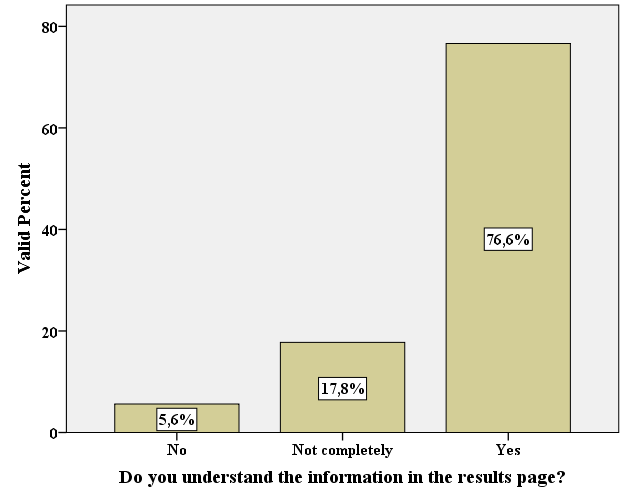
\includegraphics[height=6cm]{figs/understand.png}
\end{center}
\end{frame}

\usebackgroundtemplate{}

%--------------------------------------------------------
\begin{frame}
\frametitle{Validation Process: Ecological Validity (and III)}
\begin{center}
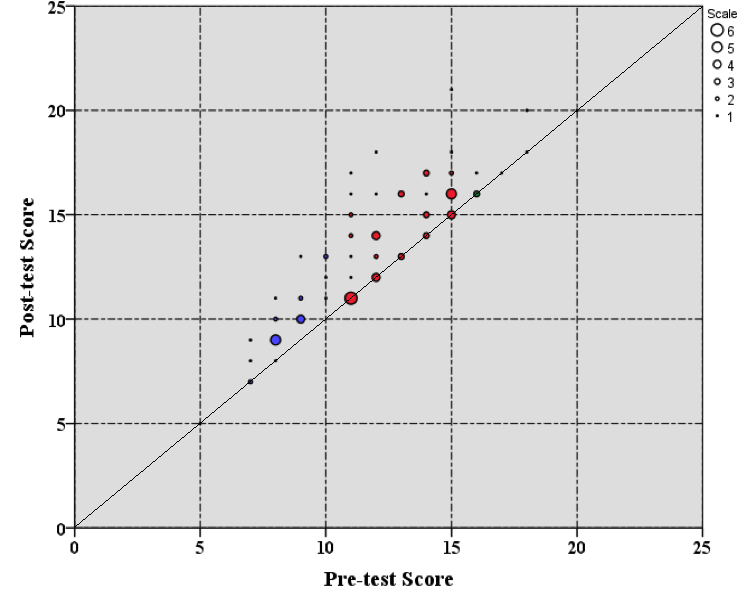
\includegraphics[height=6cm]{figs/improvement.png}
\end{center}
\end{frame}

\usebackgroundtemplate{}

%--------------------------------------------------------

\usebackgroundtemplate{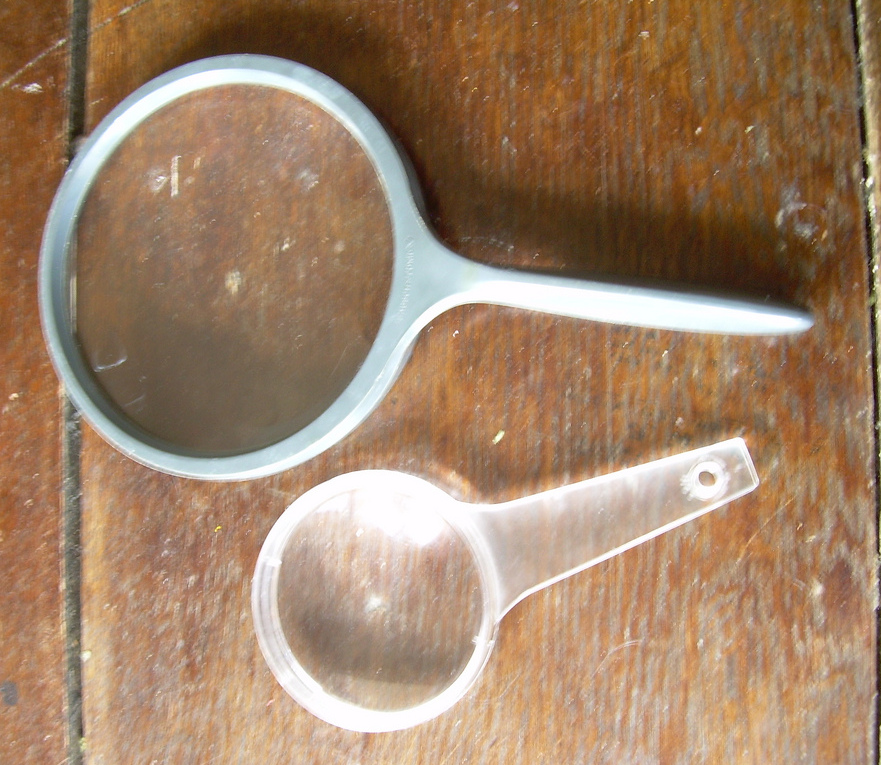
\includegraphics[width=13cm]{figs/lupa.jpg}}
%https://www.flickr.com/photos/66992990@N00/6876253645/
\begin{frame}
\frametitle{Validation Process: Convergent Validity (I)}
\begin{columns}[T]
    \begin{column}{0.8\textwidth}
     \begin{block}{Convergent validity}
     \begin{itemize}
      \item Comparison of the evaluations provided by Dr. Scratch with other measurements of similar constructs
      \begin{itemize}
       \item (Human) expert evaluators
       \item Software engineering complexity metrics
       \item CT-test
      \end{itemize}
     \end{itemize}
    \end{block}
    \end{column}
  \end{columns}
  \vspace{\baselineskip}
  \vspace{\baselineskip}
  \hfill{\Tiny Background picture: Joanna Bourne}
\end{frame}

\usebackgroundtemplate{}
%--------------------------------------------------------

\begin{frame}
\frametitle{Validation Process: Convergent Validity (II)}
\begin{center}
\begin{center}
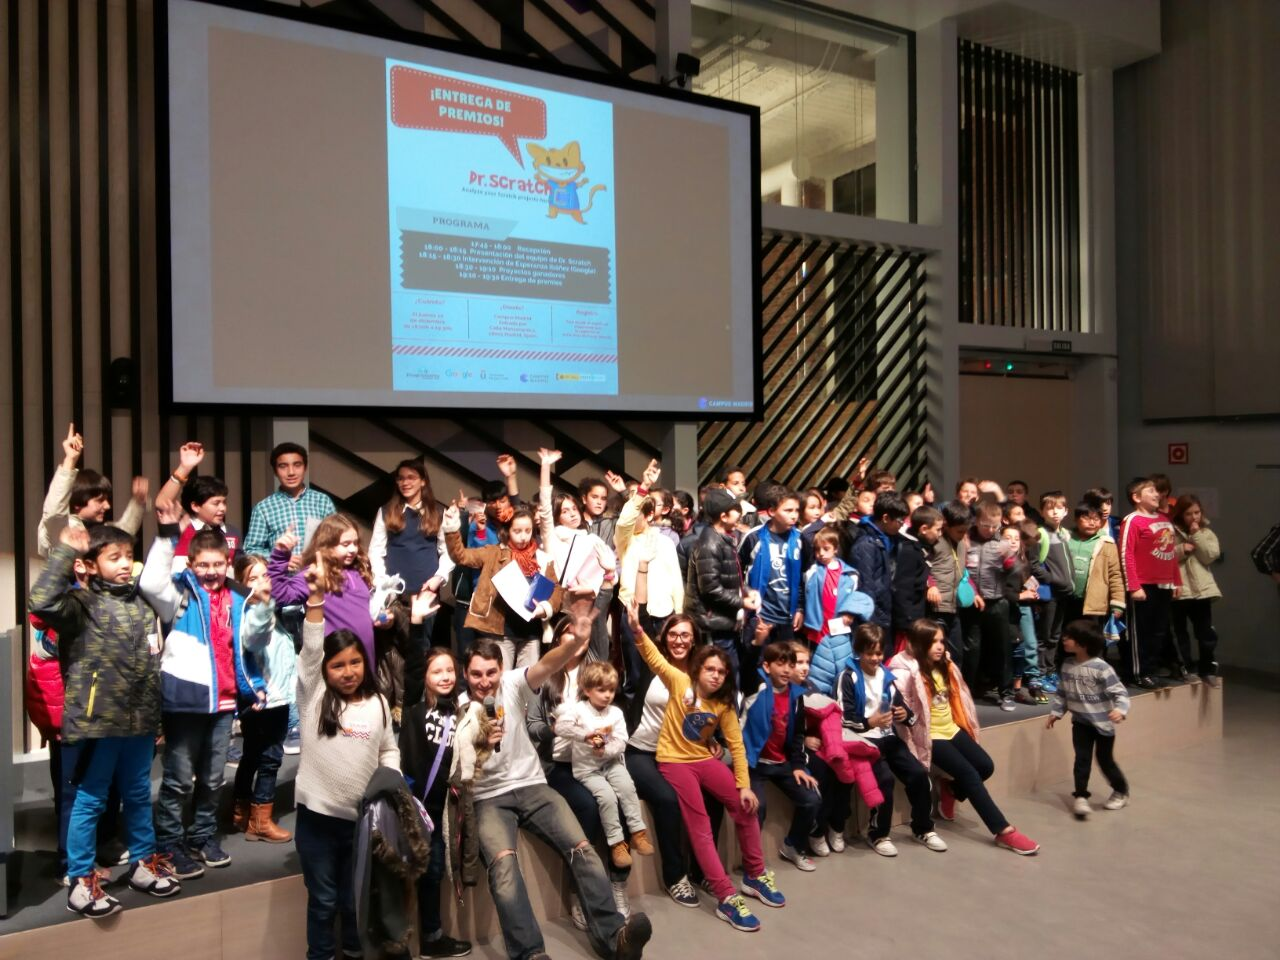
\includegraphics[height=6cm]{figs/contest.jpg}
\end{center}
Comparison with human experts - Dr. Scratch contest award ceremony at Google Campus, Madrid (Spain)
\end{center}
\end{frame}

\usebackgroundtemplate{}

%--------------------------------------------------------
\begin{frame}
\frametitle{Validation Process: Convergent Validity (III)}
\begin{center}
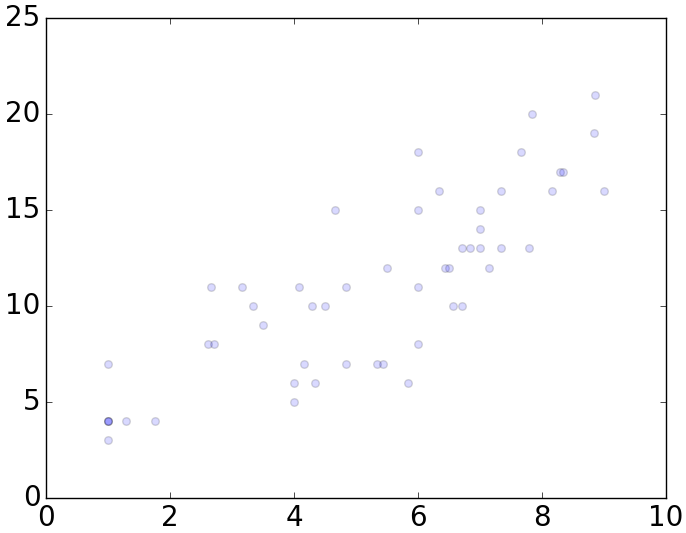
\includegraphics[height=6cm]{figs/scatterWeek1_avg.png}
\end{center}
\begin{center}
Scatter plot for experts evaluation (x-axis) and Dr. Scratch assessment (y-axis).
\end{center}

\end{frame}

\usebackgroundtemplate{}

%--------------------------------------------------------
\begin{frame}
\frametitle{Validation Process: Convergent Validity (IV)}
\begin{center}
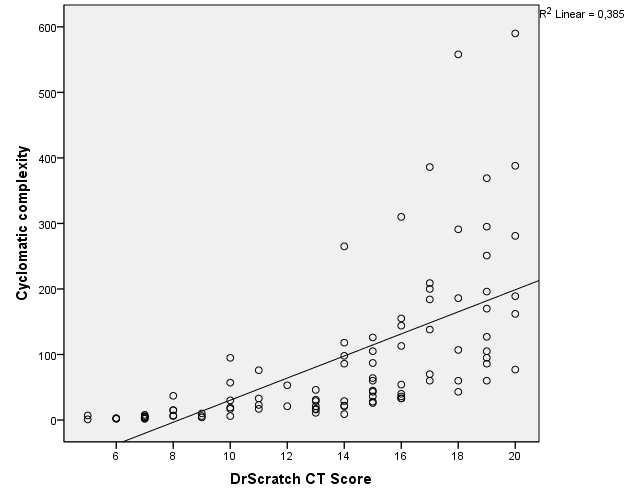
\includegraphics[height=6cm]{figs/CC.png}
\end{center}
\begin{center}
Scatter plot for Dr. Scratch assessment (x-axis) and Cyclomatic Complexity (y-axis).
\end{center}
\end{frame}

\usebackgroundtemplate{}

%--------------------------------------------------------
\begin{frame}
\frametitle{Validation Process: Convergent Validity (V)}
\begin{center}
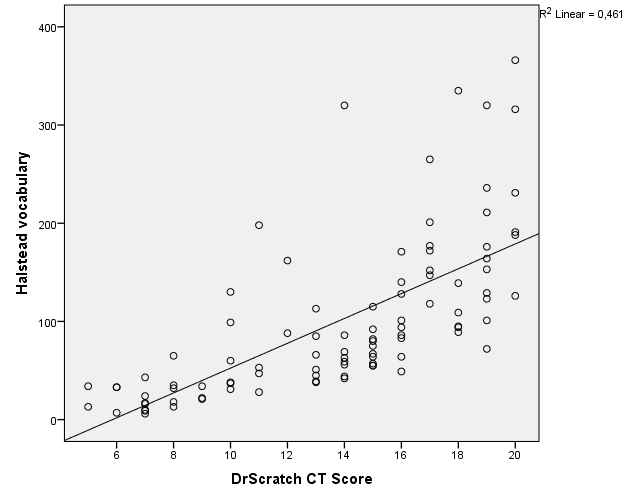
\includegraphics[height=6cm]{figs/vocabulary.png}
\end{center}
\begin{center}
Scatter plot for Dr. Scratch assessment (x-axis) and Halstead's vocabulary (y-axis).
\end{center}
\end{frame}

\usebackgroundtemplate{}

%--------------------------------------------------------
\begin{frame}
\frametitle{Validation Process: Convergent Validity (VI)}
\begin{center}
\begin{center}
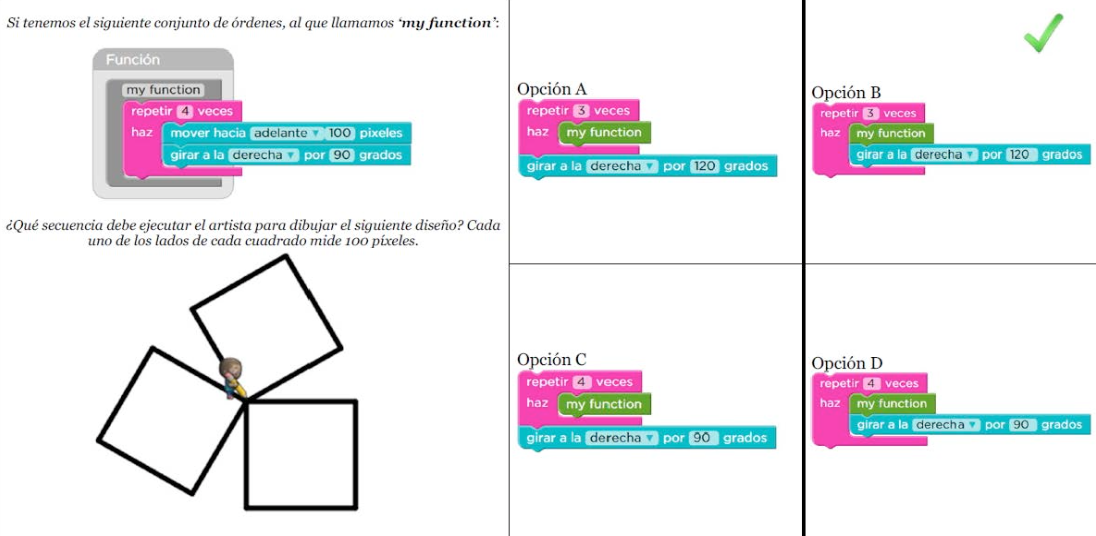
\includegraphics[height=4.5cm]{figs/tpcitem.png}
\end{center}
One of the CT-test items
\end{center}
\end{frame}

\usebackgroundtemplate{}

%--------------------------------------------------------
\begin{frame}
\frametitle{Validation Process: Convergent Validity (and VII)}
\begin{center}
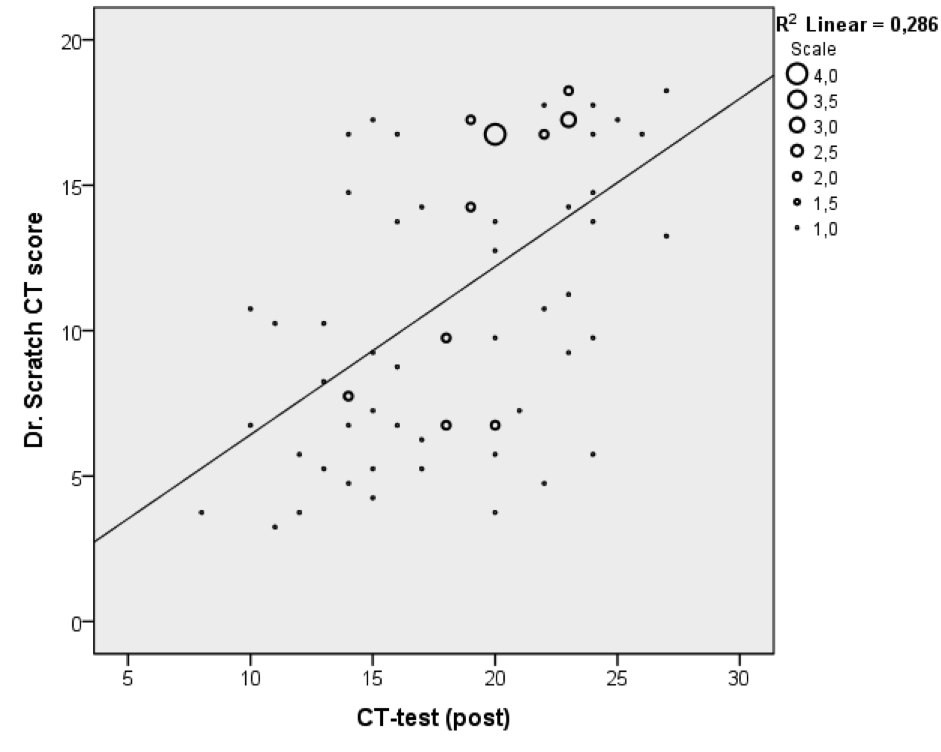
\includegraphics[height=6cm]{figs/tpc.png}
\end{center}
\begin{center}
Scatter plot for Dr. Scratch assessment (x-axis) and CT-test (y-axis).
\end{center}
\end{frame}

\usebackgroundtemplate{}


%--------------------------------------------------------

\usebackgroundtemplate{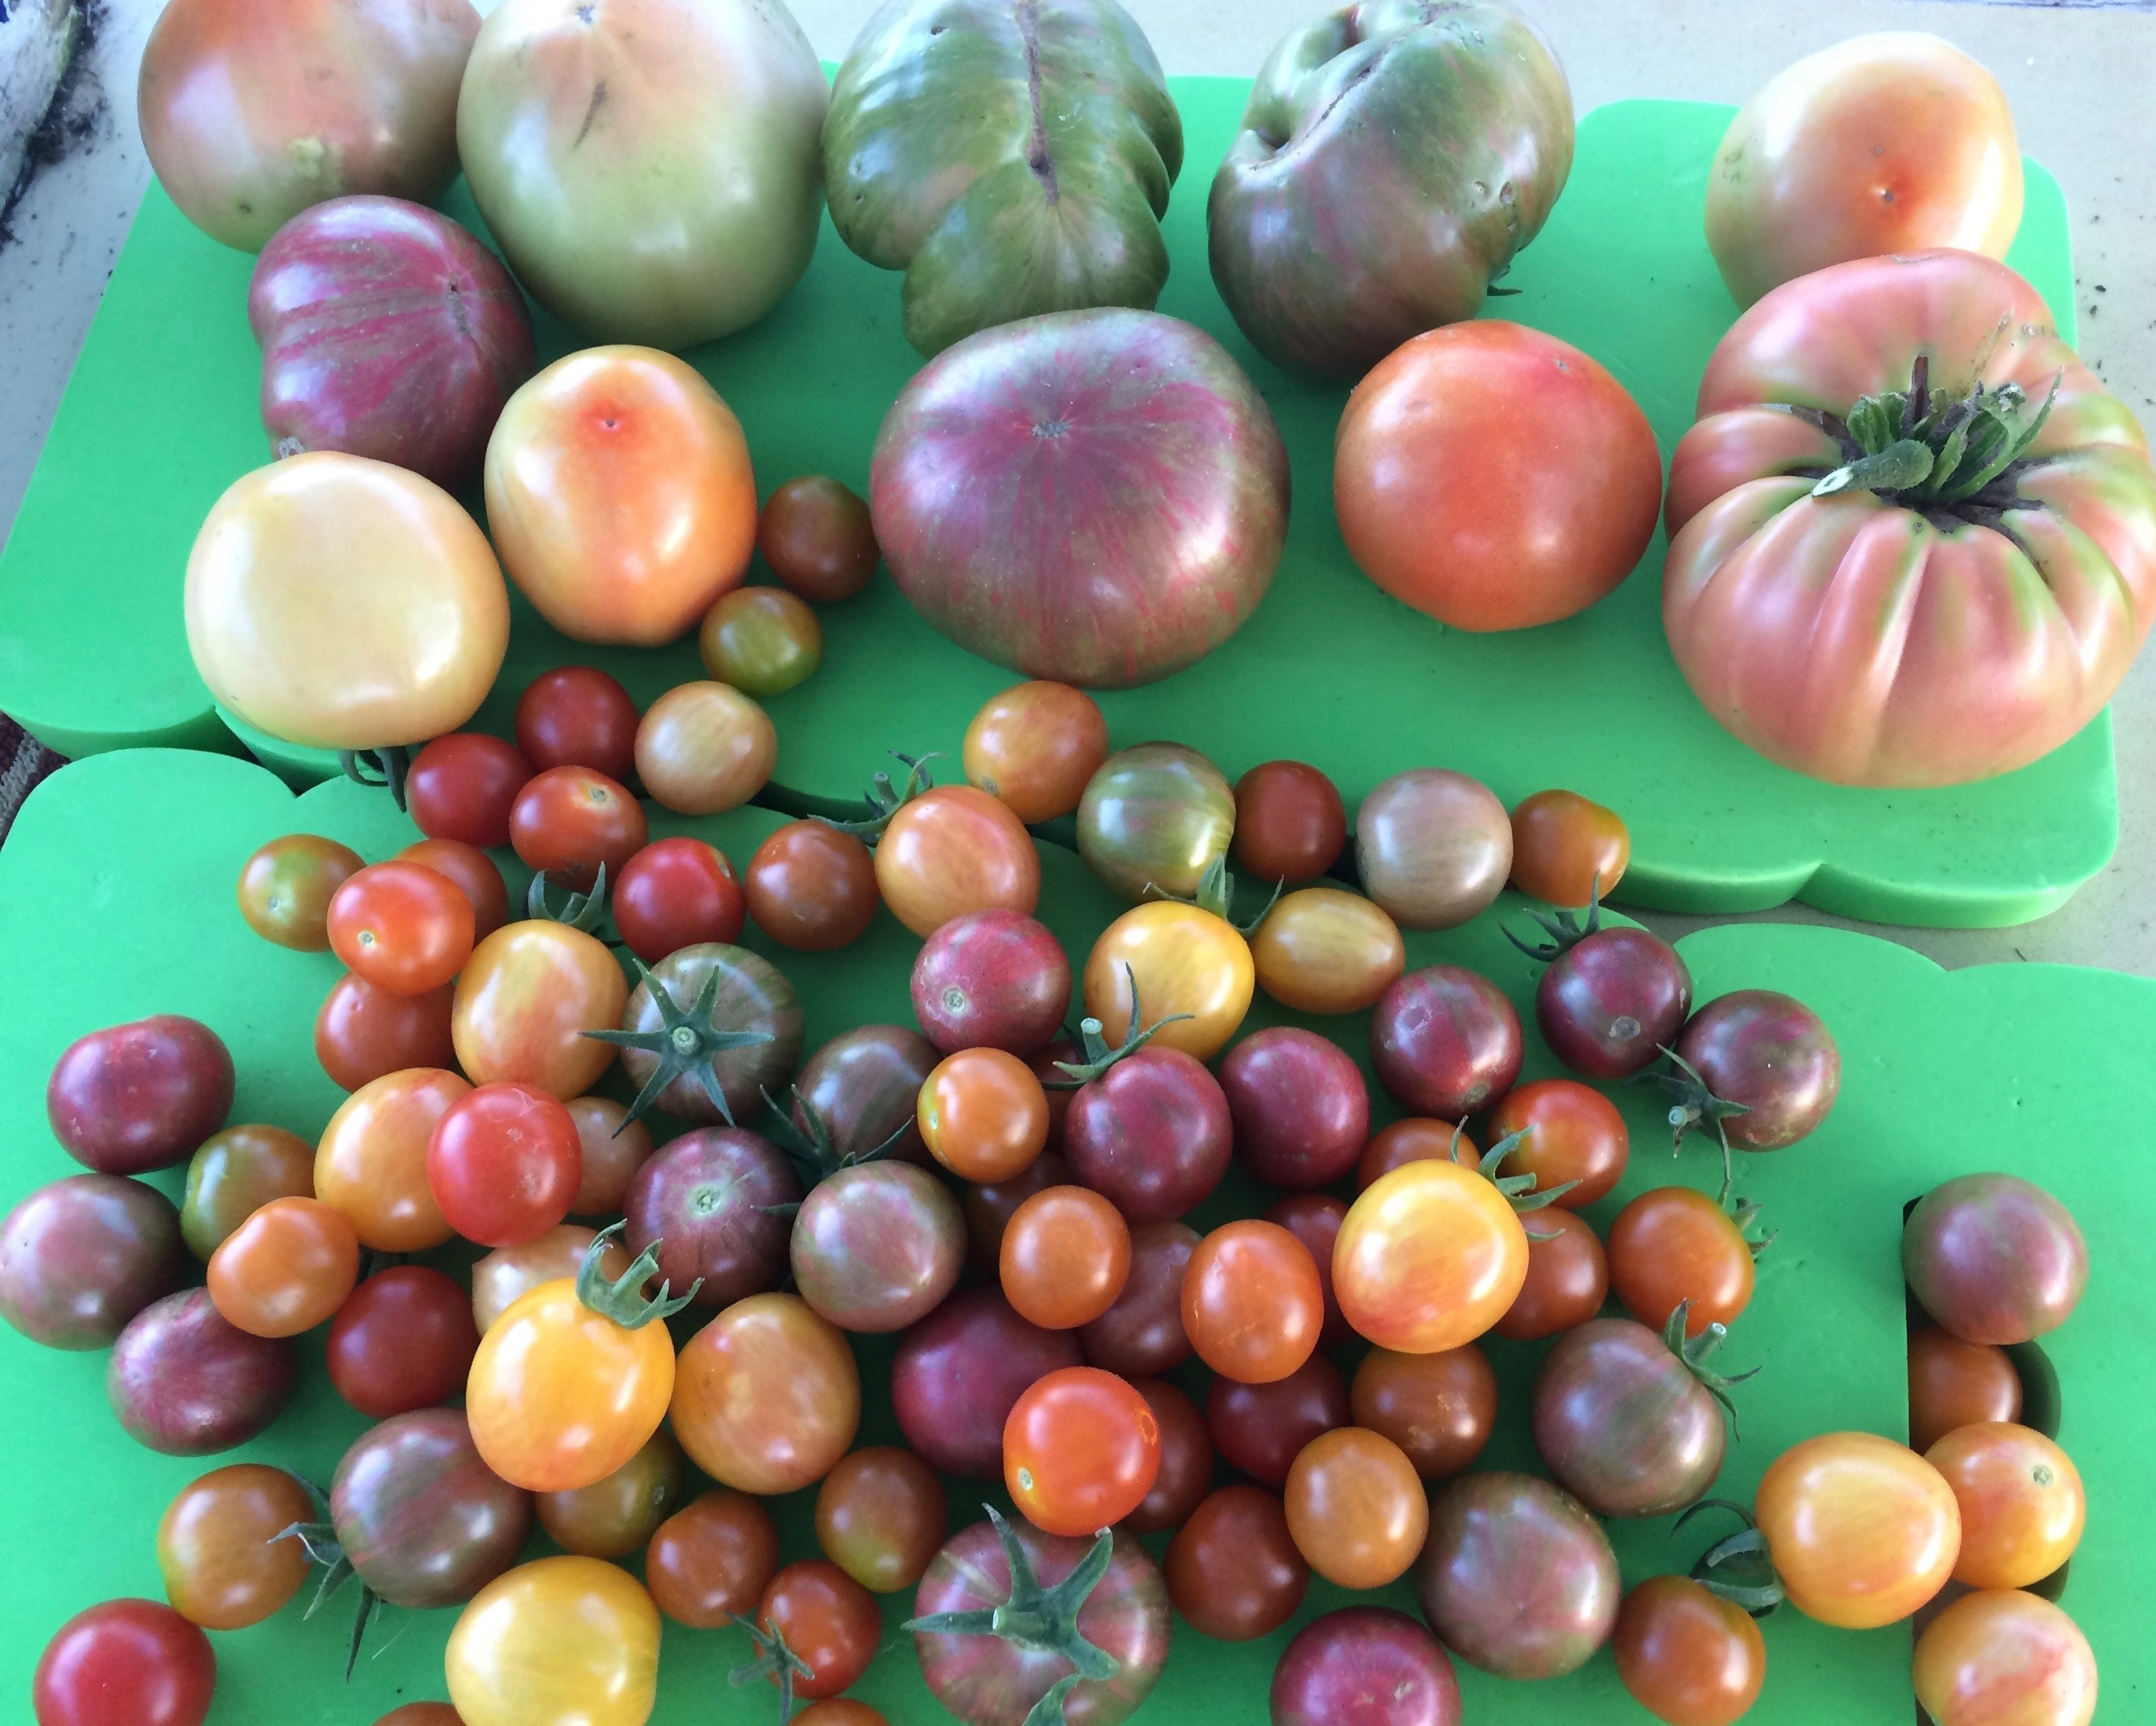
\includegraphics[width=13cm]{figs/tomates.jpg}}
%https://unsplash.com/photos/fW_ctfz1yWg
\begin{frame}
\frametitle{Validation Process: Discriminant Validity (I)}
\begin{columns}[T]
    \begin{column}{0.8\textwidth}
     \begin{block}{Discriminant validity}
     \begin{itemize}
      \item Projects shared in the Scratch repository are categorized under one or more project types: games, animations, music, art and stories. 
      \item Is Dr. Scratch able to detect differences in the CT dimensions developed when programming different types of Scratch projects?
     \end{itemize}
    \end{block}
    \end{column}
  \end{columns}
  \vspace{\baselineskip}
  \vspace{\baselineskip}
  \hfill{\Tiny Background picture: Bodie Pyndus}
\end{frame}

\usebackgroundtemplate{}
%--------------------------------------------------------

\begin{frame}
\frametitle{Validation Process: Discriminant Validity (and II)}
\begin{center}
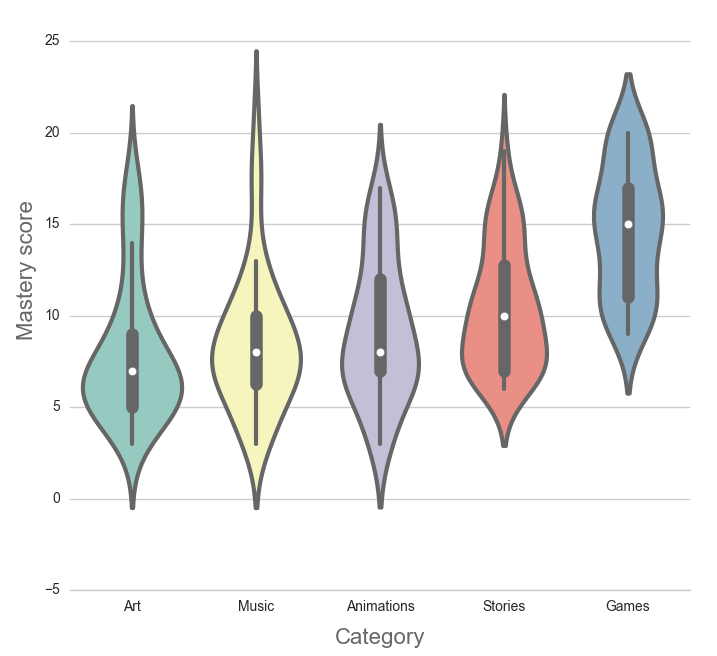
\includegraphics[height=6cm]{figs/violin.png}
\end{center}
\end{frame}

\usebackgroundtemplate{}

%--------------------------------------------------------

\usebackgroundtemplate{
\includegraphics[width=14.5cm]{figs/trust.jpg}}
%https://www.flickr.com/photos/jmennens/5085536363/
\begin{frame}
\frametitle{Validation Process: Face Validity (I)}
\begin{columns}[T]
    \begin{column}{0.8\textwidth}
     \begin{block}{Face validity}
     \begin{itemize}
      \item Educators won't use the tool unless they feel that Dr. Scratch measures what it promises (i.e. assessing CT)
      \item Over 400 teacher who participate in a 40-hours Scratch coding training course have been surveyed
     \end{itemize}
    \end{block}
    \end{column}
  \end{columns}
  \vspace{\baselineskip}
  \vspace{\baselineskip}
  \hfill{\Tiny Background picture: janmennens}
\end{frame}

\usebackgroundtemplate{}
%--------------------------------------------------------

\begin{frame}
\frametitle{Validation Process: Face Validity (and II)}
\begin{center}
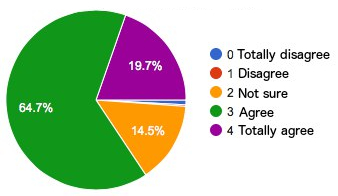
\includegraphics[height=5cm]{figs/survey.jpg}
\end{center}
\begin{center}
The CT score provided by Dr. Scratch is accurate 
\end{center}

\end{frame}

\usebackgroundtemplate{}

%--------------------------------------------------------

\usebackgroundtemplate{
\includegraphics[width=15cm]{figs/puzzle.jpg}}
%https://www.flickr.com/photos/jennyrotten/11785735774/
\begin{frame}
\frametitle{Validation Process: Factorial Validity}
\vspace{\baselineskip}
\vspace{\baselineskip}
\begin{columns}[T]
    \begin{column}{0.8\textwidth}
     \begin{block}{Factorial validity}
     \begin{itemize}
      \item Study potential relationships between the CT dimensions assessed by Dr. Scratch
      \item Simplification of the feedback report?
     \end{itemize}
    \end{block}
    \end{column}
  \end{columns}
  \vspace{\baselineskip}
  \vspace{\baselineskip}
  \hfill{\Tiny Background picture: jennyrotten}
\end{frame}

\usebackgroundtemplate{}
%--------------------------------------------------------


%\usebackgroundtemplate{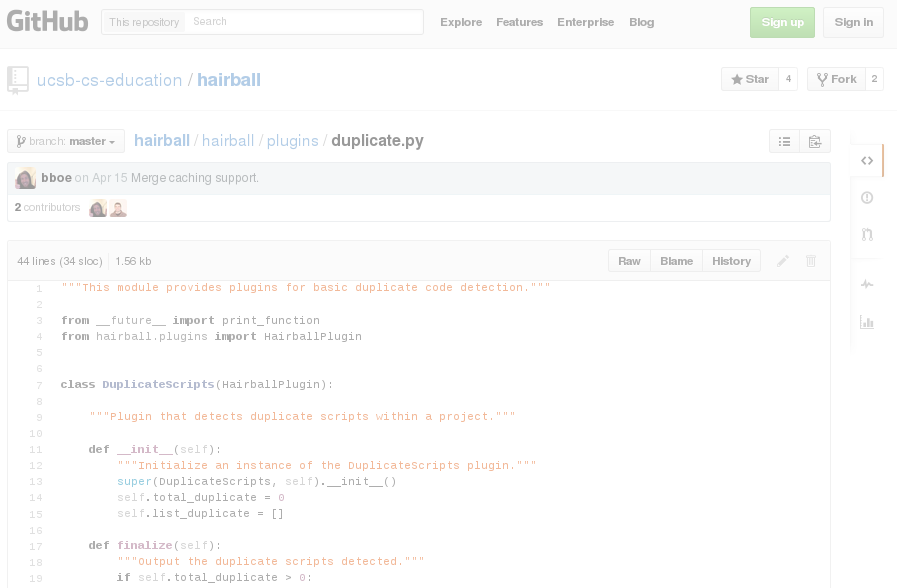
\includegraphics[width=13cm,height=9.2cm]{figs/plugins.png}}
% background: http://25.media.tumblr.com/b83aa72682992ab34b8ce7e61c0cb7f9/tumblr_menxc7qcq61ryin08o1_r1_1280.jpg
\usebackgroundtemplate{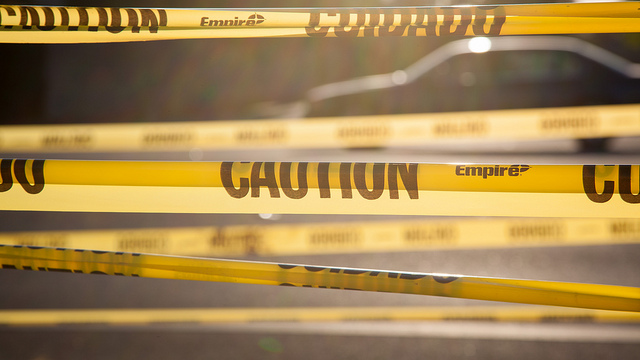
\includegraphics[width=16cm]{figs/caution.jpg}}
\begin{frame}
\frametitle{Limitations}
\begin{columns}[T]
    \begin{column}{0.8\textwidth}
     \begin{block}{Teachers should not rely exclusively on Dr. Scratch}
\begin{itemize}
  \item Fundamental CT skills not assessed: debugging and remixing.
  \item Functionality or creativity not evaluated.
  \item Portfolio analysis would be more accurate.
\end{itemize}
    \end{block}
    \end{column}
  \end{columns}
\vspace{\baselineskip}
\vspace{\baselineskip}
\hfill{\Tiny Background picture:  Robert Couse-Baker}
\end{frame}

\usebackgroundtemplate{}

%--------------------------------------------------------

\usebackgroundtemplate{
\includegraphics[width=13cm]{figs/future.png}}

\begin{frame}
\frametitle{Future Work}

\begin{enumerate}
  \item User accounts
  \item Teacher dashboard
  \item Organization dashboard
\end{enumerate}
\vspace{\baselineskip}
\vspace{\baselineskip}
\hfill{\Tiny Background picture: Simon Cunningham }

\end{frame}

\usebackgroundtemplate{}
%--------------------------------------------------------

\usebackgroundtemplate{
\includegraphics[width=13cm]{figs/take-away.jpg}}
% background: http://2.bp.blogspot.com/-78Eh4TBpdtU/UPw7ULV73PI/AAAAAAAAHAE/6DQfvPNCo-Y/s1600/8723052-stylized-red-stamp-showing-the-term-take-away-all-on-white-background.jpg

\begin{frame}
\frametitle{Links with Software Evolution (I)}
\begin{center}
\Large{\bf Tools like Dr. Scratch offer the possibility of easily tracking learners progression and projects evolution, both in terms of software complexity and presence of \emph{bad smells}}
\end{center}
\end{frame}

\usebackgroundtemplate{}

%--------------------------------------------------------


\begin{frame}
\frametitle{Links with Software Evolution (II)}
\begin{center}
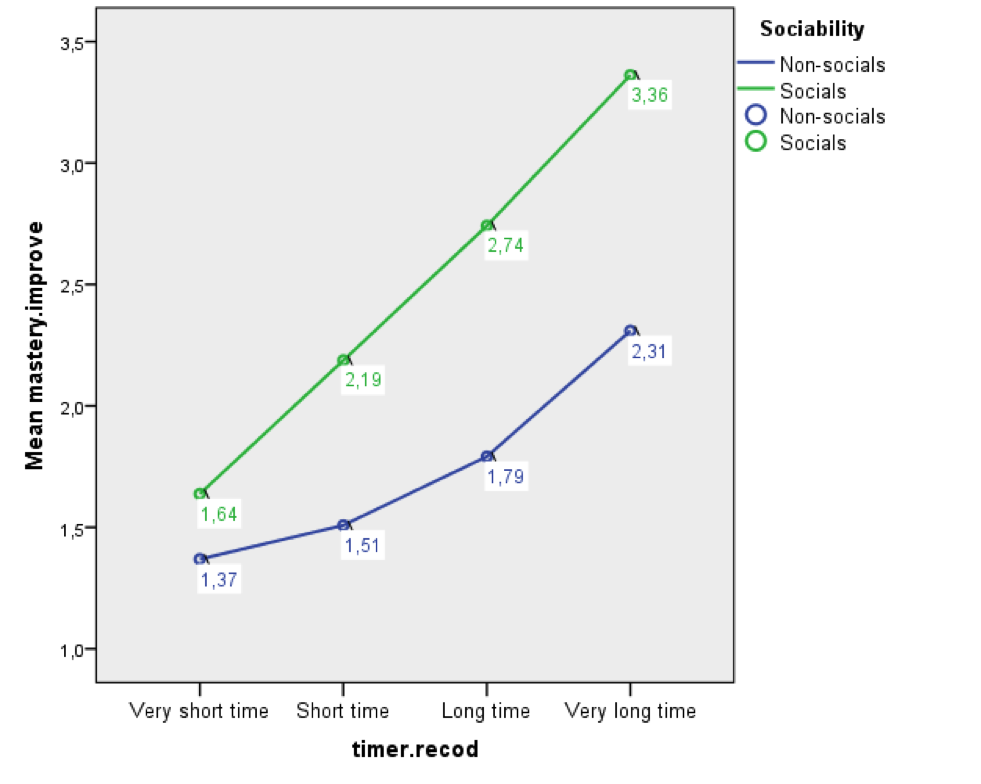
\includegraphics[height=5cm]{figs/social.png}
\end{center}
\begin{center}
\footnotesize Examining the Relationship between Socialization and Improved Software Development Skills in the Scratch Code Learning Environment. Moreno-Le�n J., Robles G. \& Rom�n-Gonz�lez M. Journal of Universal Computer Science 22 (12), pages 1533-1557, 2016.
\end{center}
\end{frame}

\usebackgroundtemplate{}

%--------------------------------------------------------

\begin{frame}
\frametitle{Links with Software Evolution (and III)}
\begin{center}
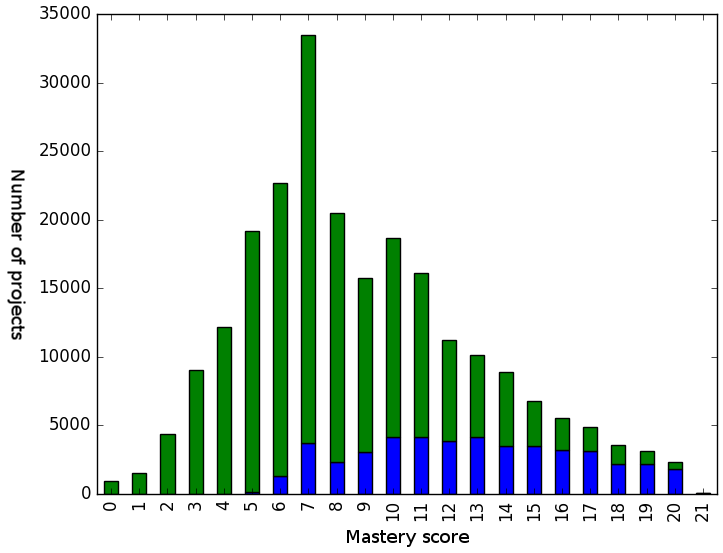
\includegraphics[height=5cm]{figs/clones.png}
\end{center}
\begin{center}
\footnotesize Software clones in scratch projects: on the presence of copy-and-paste in computational thinking learning. Robles, G., Moreno-Le\'on, J., Aivaloglou, E., \& Hermans, F. In Software Clones (IWSC), 2017 IEEE 11th International Workshop on (pp. 1-7).
\end{center}
\end{frame}

\usebackgroundtemplate{}

%--------------------------------------------------------
\usebackgroundtemplate{
\includegraphics[width=13cm]{figs/books.jpg}}
% http://www.aspa-usa.org/wp-content/uploads/2015/06/books.jpg
\begin{frame}
\frametitle{Learn more}
\begin{center}
\scriptsize
\begin{columns}[T]
    \begin{column}{1\textwidth}
     \begin{block}{Dr. Scratch references}
       \begin{itemize}
	 \item Moreno, J., \& Robles, G. (2014). Automatic detection of bad programming habits in scratch: A preliminary study. In \textit{Frontiers in Education Conference (FIE), 2014 IEEE} (pp. 1-4). IEEE.
	 \item Moreno-Le\'on, J., Robles, G, \& Roman-Gonz\'alez, M. (2015). Dr. Scratch: Automatic Analysis of Scratch Projects to Assess and Foster Computational Thinking. \textit{RED. Revista de Educaci�n a Distancia, 15}(46).
	 \item Moreno-Le\'on, J., Robles, G, \& Roman-Gonz\'alez, M. (2016). Comparing computational thinking development assessment scores with software complexity metrics. In \textit{Global Engineering Education Conference (EDUCON), 2016 IEEE} (pp. 1040-1045). IEEE.
	 \item Moreno-Le\'on, J., Roman-Gonz\'alez, M., Harteveld, C. \& Robles, G. (2017). On the Automatic Assessment of Computational Thinking Skills: A Comparison with Human Experts. In \textit{Proceedings of the 2017 CHI Conference Extended Abstracts on Human Factors in Computing Systems}. (pp. 2788-2795). ACM.
       \end{itemize}
    \end{block}
    \end{column}
  \end{columns}
\end{center}
\end{frame}

\usebackgroundtemplate{}

%--------------------------------------------------------
%\begin{frame}
%\frametitle{GSyC/LibreSoft}

%\begin{figure}[t!]
%\begin{center}
%\includegraphics[width=11cm]{figs/libresoft.jpg}
%\end{center}
%\label{fig:libresoft}
%\end{figure}

%\begin{center}
%The GSyC/LibreSoft research team at URJC (Madrid).
%\end{center}

%\end{frame}

%--------------------------------------------------------
%\begin{frame}
%\frametitle{Our work at GSyC/LibreSoft}

%\begin{figure}[t!]
%\begin{center}
%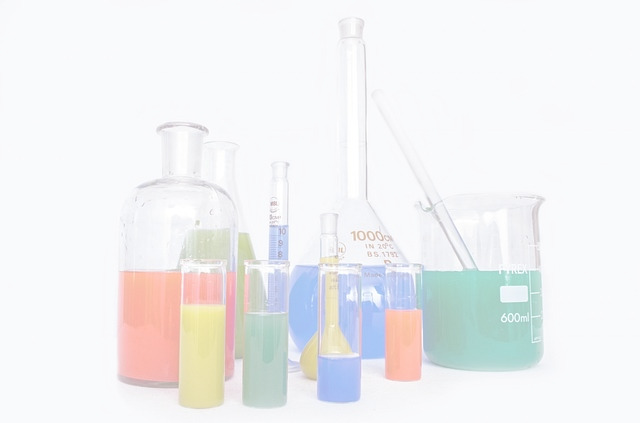
\includegraphics[width=2.5cm]{figs/research}
% http://www.memphis.edu/crow/images/research_2.jpg
%\hspace{0.1cm}
%\includegraphics[width=2.5cm]{figs/teaching}
% http://2.bp.blogspot.com/_uxgwfriLwSo/TOWDr8IjaLI/AAAAAAAABLM/d7H-G5jIq-c/s1600/teaching.gif
%\hspace{0.1cm}
%\includegraphics[width=2.5cm]{figs/development}
% http://www.vidadigitalradio.com/wp-content/uploads/2009/04/hackers_cartoons.jpg
%\hspace{0.1cm}
%\includegraphics[width=2.5cm]{figs/promotion}
% http://bloggeate.com/wp-content/uploads/2011/04/como-promocionar-tu-blog.jpg
%\end{center}
%\label{fig:whatwedo}
%\end{figure}

%\begin{center}
%GSyC/LibreSoft's tasks: research, teaching, development, promotion of free software.

%\end{center}
%\end{frame}

\usebackgroundtemplate{}

%--------------------------------------------------------
\frame{
\maketitle
\begin{center}

\includegraphics[width=2cm]{format/libresoft-logo}
\hspace{0.5cm}

\includegraphics[width=5cm]{format/gsyc-urjc}
\vspace{0.5cm}

\includegraphics[width=3cm]{format/emadrid.png}
\end{center}
}

\end{document}
